\documentclass[11pt]{article}
\usepackage{times}
\usepackage{amsmath,amsthm,amssymb,setspace,enumitem,epsfig,titlesec,verbatim,color,array,eurosym,multirow}
\usepackage[sort&compress]{natbib}
\usepackage[footnotesize,bf]{caption}
\usepackage[margin=2.5cm, includefoot, footskip=30pt]{geometry}
\usepackage{standalone}
\usepackage{tikz}
\usepackage{subcaption}
\usepackage{hyperref}
\usepackage{tabularx}
\usepackage{booktabs}
\usepackage{blkarray}
\usepackage[ruled,vlined]{algorithm2e}
\smallskip % Erlaubt kleine Abstaende zwischen Paragraphen, falls es dem Seitenlayout hilft
\renewcommand{\baselinestretch}{1.3}
\newcommand{\R}{\mathbb{R}}

\definecolor{darkblue}{rgb}{0,0,.8}
\definecolor{darkgreen}{rgb}{0,0.5,0.1}
\newcommand{\matlabfunc}[1]{\textcolor{darkblue}{#1}}
\newcommand{\matlabcomment}[1]{\textcolor{darkgreen}{#1}}
\newcommand{\christian}[1]{\textcolor{blue}{\textbf{CH}: #1}}
\newcommand{\alex}[1]{\textcolor{red}{\textbf{AL}: #1}}

%% Adding shortcut commands to refer to our figures %%
\newcommand{\FigEvoProc}{{\bf Fig.~1}} \newcommand{\FigInvAnalysis}{{\bfFig.~2}} \newcommand{\FigResultsOverPara}{{\bf Fig.~3}}


\titleformat{\section}{\sffamily \fontsize{12}{14}\bfseries}{\thesection}{1em}{}
\titleformat{\subsection}{\sffamily
\fontsize{11.5}{11.5}\bfseries}{\thesubsection}{1em}{}

\usepackage{tikz}
\usetikzlibrary{arrows}

\tikzset{treenode/.style = {align=center, inner sep=0pt, text centered,
  font=\sffamily}, arn_n/.style = {treenode, circle, white,
  font=\sffamily\bfseries, draw=black, inner sep=-6pt, fill=black, text
  width=1.5em},% arbre rouge noir, noeud noir
  arn_r/.style = {treenode, circle, red, text width=1.5em, very thick, inner
    sep=4pt},% arbre rouge noir, noeud rouge
  arn_x/.style = {treenode, rectangle, draw=black, minimum width=0.5em, minimum
    height=0.5em}% arbre rouge noir, nil
}

\newtheoremstyle{plainCl1}% name
{9pt}%      Space above, empty = 'usual value'
{9pt}%      Space below
{\it}% 	   Body font
{}%         Indent amount (empty = no indent, \parindent = para indent)
{\bfseries}% Thm head font
{.}%        Punctuation after thm head
{0.2cm}% Space after thm head: \newline = linebreak
{}%         Thm head spec

\newtheoremstyle{plainCl2}% name
{9pt}%      Space above, empty = 'usual value'
{9pt}%      Space below
{\it}% 	   Body font
{}%         Indent amount (empty = no indent, \parindent = para indent)
{\bfseries}% Thm head font
{$'$.}%        Punctuation after thm head
{0.2cm}% Space after thm head: \newline = linebreak
{}%         Thm head spec

\newcommand{\splitatcommas}[1]{%
  \begingroup
  \begingroup\lccode`~=`, \lowercase{\endgroup \edef~{\mathchar\the\mathcode`,
    \penalty0 \noexpand\hspace{0pt plus 1em}}%
  }\mathcode`,="8000 #1%
  \endgroup
}

\theoremstyle{plainCl1}
\newtheorem{Claim}{Claim}
\newtheorem{Thm}{Theorem}
\newtheorem{Prop}{Proposition}
\newtheorem*{Lem}{Lemma}
\newtheorem{Cor}{Corollary}
\newtheorem*{Def}{Definition}

\theoremstyle{plainCl2}
\newtheorem{Claim2}{Claim}

\title{\bf  \sffamily \LARGE Evolution of cooperation among individuals with
limited payoff memory\\}
\date{}
\author{Nikoleta E. Glynatsi, Christian Hilbe, Alex McAvoy}

\begin{document}
\maketitle

\begin{abstract}
Repeated games are vastly used in evolutionary game theory to explain cooperation
in a variety of environments. Although existing models have shaped our
understanding of human cooperation they often work with idealized assumptions.
In an evolutionary process, individuals imitate other individuals of the
population based on their fitness. It is commonly assumed that an individual
computes their fitness after interacting with a representative sample of the
population and remembering all the interactions they participated in. In real
life we do not always remember all our interactions, instead we rather recall
our most recent ones.

Here we introduce a framework that allows individuals to estimate their fitness
based on a minimum of social information. We explore the difference between our
framework and the classical framework using the iterated prisoner's dilemma. We
show that individuals relying on a single set of information tend to adopt less
generous strategies and they achieve less cooperation than in the classical
scenario. Although strategies in the latter scenario become more cooperative
with increasing benefits, those in the former remain unchanged. We further
explore scenarios where individuals are granted slightly more information, and
our observations indicate that these individuals can attain higher levels of
cooperation.

\end{abstract}

\section{Introduction}

Evolutionary game theory~\cite{smith1982evolution, hofbauer1998evolutionary,
nowak:Nature:2004, hauert2005game} describes the evolutionary dynamics of
populations consisting of different types of interacting individuals. In the
last two decades the interest of the field has shifted to the analysis of
stochastic finite population dynamics in preference to traditional approaches
such as the replicator dynamics~\cite{hofbauer:JTB:1979, taylor:MATHBIO:1978}.
This is especially true in the topic of cooperation~\cite{hilbe:PNAS:2013,
hilbe:Nature:2018,glynatsi:SCR:2020, ohtsuki:Nature:2006, nowak:Science:2006,
murase:ScientificReports:2020}. In stochastic evolutionary dynamics
disadvantageous mutants have a small yet non-zero probability to reach fixation
and this can lead to fundamental changes in the results. As shown
in~\cite{nowak:Nature:2004}, using such dynamics a single cooperative strategy
can invade a population of defectors without any special modifications in
comparison to traditional approaches that one has to consider spatial
structure~\cite{nowak:Nature:1992} or when payoffs are subject to aggregate
shocks~\cite{fudenberg:JET:1992}.

Stochastic evolutionary dynamics model a finite population. Each
time step of the process consists of three phases; (1) the \textit{mutation
phase} (2) the \textit{game phase} (3) the \textit{update phase}. In the
mutation phase one individual from the population is chosen to switch to a new
mutant strategy with a probability \(\mu\). In the game phase individuals are
randomly matched with other individuals in the population, and they engage in a
repeated game where each subsequent turn occurs with a fixed probability
\(\delta\). The updating phase depends on the process. Two classes of
finite stochastic processes have been used extensively: (i) fitness-based
processes in which an individual chosen proportional to fitness reproduces and
the offspring replaces a randomly chosen individual~\cite{nowak:Nature:2004} or
(ii) \textit{pairwise comparison processes} in which a pair of individuals is
chosen and subsequently one of these individuals may adopt the strategy of the
other~\cite{traulsen2007pairwise}.

Like all theoretical models, finite stochastic processes rest on a
set of assumptions. Namely, in the game phase it is assumed that players use
strategies with finite memory~\cite{Nowak1992tit, Baek2016}. For example, in a
repeated game between two individuals the actions of the players in each turn
are often determined by the action of the co-players in the previous turn~\cite{Nowak1992tit}. This
assumption is common as it allows for an explicit calculation of the players'
payoffs~\cite{sigmund2010calculus}. In addition, it is
assumed that individuals play many times and with all other players before
reproduction takes place. So that in the updating phase the updating payoffs,
or fitness, of individuals is given by the average payoffs of an
infinitely repeated game against every member of the population.

These two assumptions create a curious inconsistency; a player with a finite
memory (in the game stage) can recall infinite information regarding their
interactions and each interaction's outcomes in the update stage. Prior research
has examined the effects of constraining the interactions an individual has.
Either by letting individuals have a stochastic number of
interactions~\cite{roca:PhysicalReview:2006, sanchez:JTB:2005,
Traulsen:JTB:2007} or by only allowing for a single
interaction~\cite{Woelfing:JTB:2009}. However, these studies have not accounted
for the use of strategies with finite memory. Moreover, no previous research has
explored the effect of restricting not only the number of interactions, but also
the amount of information available about each interaction. To this end, we
propose a framework in which individuals, similar to the decisions at each turn,
estimate their fitness based on a minimum of information.

We first consider two extreme scenarios, the classical scenario where an individual
has a perfect memory of all their interactions and the alternative scenario of
limited memory where individuals update their strategies only based on the very
last payoff they obtained. We demonstrate the effects of limited payoff
memory using a pairwise comparison process and the well studied game of the
prisoner's dilemma~\cite{glynatsi:HSSC:2021}. We observe that individuals with
limited payoff memory tend to adopt less generous strategies. We obtain similar
results when we consider that individuals update their strategies based on more
information. More specifically, up to the last two payoffs they obtained when
interacting with up to two different members of the population.

\section{Model Setup}\label{section:model}

A pairwise comparison process~\cite{traulsen2007pairwise} starts with assigning all
individuals of the population the same strategy. Thenceforth each elementary time step of
the process consists of the mutation phase, the game phase and the update phase.
In the game phase individuals are matched in pairs and that they participate in
a repeated 2 person donation game; a special case of the prisoner's dilemma. In
the donation game there are two actions: cooperation (\(C\)) and defection
(\(D\)). By cooperating a player provides a benefit \(b\) to the other player at
their cost \(c\), with \(0 < c < b\). Thus the payoffs for a player in each turn
are given by,

\begin{equation}
    \begin{blockarray}{ccc}
        & \text{cooperate} & \text{defect} \\
        \begin{block}{c(cc)}
            \text{cooperate} & b - c & -c \\
            \text{defect} & b & 0 \\
        \end{block}
    \end{blockarray}.
\end{equation}

Let \(\mathbf{u} = (b-c, -c, b, 0)\) be the round payoffs in a vector format, and let
\(\mathcal{U} = \{r, s, t, p\}\) denote the set of feasible payoffs, where \(r\)
denotes the payoff of mutual cooperation, \(s\) the sucker's payoff, \(t\) the
temptation to defect payoff, and \(p\) the punishment payoff.

In repeated games there are infinite many strategies, however, similar to the
literature we will assume that individuals use reactive strategies. A reactive
strategy considers only the previous action of the other player, and thus, a
reactive strategy \(s\) can be written as a three-dimensional vector \(s=(y, p,
q)\). The parameter \(y\) is the probability that the strategy opens with a
cooperation and \(p\), \(q\) are the probabilities that the strategy cooperates
given that the opponent cooperated and defected equivalently. The play between a
pair of reactive strategies $s_1 = (y_1, p_1, q_1)$ and $s_2 = (y_2, p_2, q_2)$
can be model as a Markov process with the transition matrix \(M\)~\cite{nowak:APC:1989},

\begin{equation}\label{eq:transition_matrix}
  M = \left[\begin{matrix} p_{1} p_{2} & p_{1} \left(1 - p_{2}\right) & p_{2} \left(1 - p_{1}\right) & \left(1 - p_{1}\right) \left(1 - p_{2}\right)\\
    p_{2} q_{1} & q_{1} \left(1 - p_{2}\right) & p_{2} \left(1 - q_{1}\right) & \left(1 - p_{2}\right) \left(1 - q_{1}\right)\\
    p_{1} q_{2} & p_{1} \left(1 - q_{2}\right) & q_{2} \left(1 - p_{1}\right) & \left(1 - p_{1}\right) \left(1 - q_{2}\right)\\
    q_{1} q_{2} & q_{1} \left(1 - q_{2}\right) & q_{2} \left(1 - q_{1}\right) & \left(1 - q_{1}\right) \left(1 - q_{2}\right)\end{matrix}\right]
\end{equation}

and the stationary vector \(\mathbf{v}(s_1,s_2)\)
which is the solution to \(\mathbf{v}(s_1,s_2) \times M 
= \mathbf{v}(s_1,s_2)\).

In the update stage two individuals are randomly selected. From the two
individuals, one  serves as the `learner' and the other as the `role model'. The
learner adopts the role model's strategy with a probability \(\rho\) given by,

\begin{equation} \label{Eq:rho}
    \rho(\pi_{L}, \pi_{RM}) = \frac{1}{1\!+\! e^{\!-\!\beta (\pi_{RM}\!-\! \pi_{L})}}.
\end{equation}

\(\pi_{L}\) and \(\pi_{RM}\) are the updating payoffs/fitness of the learner and the
role model respectively. The updating payoffs are a measure of how successful
individuals are in the current standing of the population. The parameter
\(\beta\) is known as the selection strength, namely, it shows how important the
payoff difference is when the learner is considering adopting the strategy of
the role model.

For the results presented here we assume that mutations are rare (\(\mu
\rightarrow 0\)). In fact, so rare that only two different strategies can be
present in the population at any given time. However, in the Supplementary Information
Section 9 we show that the main result holds for \(\mu \neq 0\).
The case of low mutation is vastly adopted because it allows us to explicitly
calculate the fixation probability of a newly introduced mutant. More specifically,
at each step
one individual adopts a mutant strategy randomly selected from the set of
feasible strategies. The fixation probability \(\phi_{M}\) of the mutant
strategy can be calculated explicitly as,

\begin{equation}\label{eq:appendix_fixation_probability}
    \varphi_{M} = \frac{1}{1+\sum\limits_{i=1}^{N-1}\prod\limits_k^i \frac{\lambda^-_k}{\lambda^+_k}},
\end{equation}

where \(k\) is the number of
mutants and \(\lambda^-_k, \lambda^+_k\) are the probabilities that the number of
mutants decreases and increases respectively.
Depending on the fixation probability \(\phi_{M}\) the mutant either
fixes (becomes the new resident) or goes extinct. Regardless, in the next elementary
time step another mutant strategy is introduced to the population. We iterate
this elementary population updating process for a large number of mutant
strategies and we record the resident strategies at each time step. The
probabilities \(\lambda^-_k \text{ and } \lambda^+_k\) depend on the fitness
of the mutant and the resident strategies. In the next section we
present how fitness is calculated in the cases of perfect and limited payoff memory.

\subsection{Fitness based on Perfect and Limited Payoff Memory}

In the perfect payoff memory case an individual updates based on the average payoff
against each other member of the population, otherwise known as expected payoffs. 
The payoff of a reactive strategy \(s_1\) against the reactive strategy \(s_2\)
in an infinitely repeated game ($\delta \rightarrow 1$) is explicitly
calculated as,

\[\langle\mathbf{v}(s_1,s_2),\mathbf{u}\rangle.\]

In a population of size \(N\) there are \(k\) mutants and \(N - k\) residents.
Let \(s_M =(y_M, p_M, q_M)\) and \(s_R = (y_R, p_R, q_R)\) denote the
strategies of a mutant and a resident, the expected payoffs \(\pi_R\) and
\(\pi_M\) are given by,

\begin{equation} \label{Eq:ExpPay}
  \begin{array}{lcrcr}
  \displaystyle \pi_R & = &\displaystyle \frac{N\!-\!k\!-\!1}{N-1}\cdot \langle\mathbf{v}(s_R,s_R),\mathbf{u}\rangle	&+	&\displaystyle\frac{k}{N-1}\cdot \langle\mathbf{v}(s_R,s_M),\mathbf{u}\rangle,\\[0.5cm]
  \displaystyle \pi_M & = &\displaystyle\frac{N-k}{N-1}\cdot \langle\mathbf{v}(s_M,s_R),\mathbf{u}\rangle&+	&\displaystyle\frac{k-1}{N-1}\cdot \langle\mathbf{v}(s_M,s_M),\mathbf{u}\rangle.\\
  \end{array}
\end{equation}

The probabilities that the number of mutants decreases and increases,
\(\lambda^-_k\) and \(\lambda^+_k\), in the perfect payoff memory case are
defined as,

\begin{align}\label{eq:perfect_memory_lambdas}
  \lambda^-_k \!=\!\rho(\pi_M, \pi_R) \quad \text{ and } \quad \lambda^+_k \!=\!\rho(\pi_R, \pi_M).
\end{align}

In the case of limited payoff memory we initially define the probability that a
reactive strategy receives the payoff $u\!\in\! \mathcal{U}$ in the very last
round of the game. This is given by Proposition~\ref{proposition:last_round}
(see Supplementary Information Section 2.2.1 for proof).

\begin{Prop}\label{proposition:last_round} Consider a repeated game, with
continuation probability $\delta$, between players with reactive strategies
$s_1\!=\!(y_1, p_1, q_1$)  and $s_2\!=\!(y_2,p_2,q_2)$ respectively. Then
the probability that the $s_1$ player receives the payoff $u\!\in\!
\mathcal{U}$ in the very last round of the game is given by
$v_{u}(s_1,s_2)$, as given by Equation~(\ref{Eq:LastRound}).

\begin{equation} \label{Eq:LastRound}
  \setlength{\arraycolsep}{1pt}
  \begin{array}{rcl}

  v_{r}(s_1,s_2) &= &\displaystyle (1\!-\!\delta)\frac{y_1y_2}{1\!-\!\delta^2 l_1 l_2}+\delta \frac{\Big(q_1+l_1\big((1\!-\!\delta)y_2+\delta q_2\big)\Big) \Big(q_2+l_2\big((1\!-\!\delta)y_1+\delta q_1\big)\Big)}
  {\displaystyle(1\!-\!\delta l_1l_2)(1\!-\!\delta^2 l_1 l_2)},\\[1cm]

  v_{s}(s_1,s_2) &= &\displaystyle (1\!-\!\delta)\frac{y_1\bar{y}_2}{1\!-\!\delta^2 l_1 l_2}+\delta \frac{\Big(q_1+l_1\big((1\!-\!\delta)y_2+\delta q_2\big)\Big) \Big(\bar{q}_2+\bar{r}_2\big((1\!-\!\delta)y_1+\delta p_1\big)\Big)}
  {\displaystyle(1\!-\!\delta l_1l_2)(1\!-\!\delta^2 l_1 l_2)},\\[1cm]

  v_{t}(s_1,s_2) &= &\displaystyle (1\!-\!\delta)\frac{\bar{y}_1y_2}{1\!-\!\delta^2 l_1 l_2}+\delta \frac{\Big(\bar{q}_1+\bar{r}_1\big((1\!-\!\delta)y_2+\delta p_2\big)\Big) \Big(q_2+l_2\big((1\!-\!\delta)y_1+\delta q_1\big)\Big)}
  {\displaystyle(1\!-\!\delta l_1l_2)(1\!-\!\delta^2 l_1 l_2)},\\[1cm]

  v_{p}(s_1,s_2) &= &\displaystyle (1\!-\!\delta)\frac{\bar{y}_1\bar{y}_2}{1\!-\!\delta^2 l_1 l_2}+\delta \frac{\Big(\bar{q}_1+\bar{r}_1\big((1\!-\!\delta)y_2+\delta p_2\big)\Big) \Big(\bar{q}_2+\bar{r}_2\big((1\!-\!\delta)y_1+\delta p_1\big)\Big)}
  {\displaystyle(1\!-\!\delta l_1l_2)(1\!-\!\delta^2 l_1 l_2)}.
  \end{array}
\end{equation}

In these expressions, we have used the notation $l_i:=p_i\!-\!q_i$,
$\bar{y}_i\!=\!1\!-\!y_i$, $\bar{q}_i:=1\!-\!q_i$, and
$\bar{l}_i:=\bar{p}_i\!-\!\bar{q}_i=-l_i$ for $i\!\in\!\{1,2\}$.
\end{Prop}

In the case of limited payoffs memory both the role model and the learner
estimate their fitness after interacting with a single member of the population.
At each time step there are five possible pairings. They interact with each
other with a probability \(\frac{1}{N - 1}\), and they do not interact with
other with a probability \(1 - \frac{1}{N - 1}\). In the latter case, each of
them can interact with either a mutant or a resident. Both of them interact with
a mutant with a probability $\frac{(k-1)(k-2)}{(N-2)(N-3)}$ and both interact
with a resident with a probability $\frac{(N-k-1)(N-k-2)}{(N-2)(N-3)}$. The last
two possible pairings are that either of them interacts with a resident whilst
the other interacts with a mutant, and this happens with a probability
$\frac{(N-k-1)(k-1)}{(N-2)(N-3)}$. We define the probability that the randomly
chosen resident obtained a payoff of $u_R$ in the last round of his respective
game, and that the mutant obtained a payoff of $u_M$ as $x(u_R,u_M)$.

\begin{equation}\label{eq:Chi}
\setlength{\arraycolsep}{1pt}
\begin{array}{llrl}
x(u_R,u_M)	 &=&\displaystyle \frac{1}{N\!-\!1}\cdot  &v_{u_R}(s_R,s_M)\cdot 1_{(u_R,u_M)\in \mathcal{U}^2_F}\\[0.5cm]
&+	
&\displaystyle \left(1\!-\!\frac{1}{N\!-\!1}\right)  
&\left[ \frac{k\!-\!1}{N\!-\!2}\frac{k\!-\!2}{N\!-\!3} v_{u_R}(s_R,s_M) v_{u_M}(s_M,s_M) + 
 \frac{k\!-\!1}{N\!-\!2}\frac{N\!-\!k\!-\!1}{N\!-\!3} v_{u_R}(s_R,s_M) v_{u_M}(s_M,s_R)\right.\\[0.5cm]
&&&\left. +\frac{N\!-\!k\!-\!1}{N\!-\!2}\frac{k\!-\!1}{N\!-\!3} v_{u_R}(s_R,s_R) v_{u_M}(s_M,s_M) + 
 \frac{N\!-\!k\!-\!1}{N\!-\!2}\frac{N\!-\!k\!-\!2}{N\!-\!3} v_{u_R}(s_R,s_R) v_{u_M}(s_M,s_R)\right].
\end{array}
\end{equation}

The probability that the number of mutants increases and decreases by one in the
case of limited payoff memory are now given by,

\begin{align}\label{eq:limited_memory_lambdas}
\lambda^+_k=\frac{N\!-\!k}{N} \cdot \frac{k}{N} \cdot \sum_{u_{R},u_{M}\in\mathcal{U}} x(u_{R},u_{M}) \rho(u_{R},u_{M}) \quad \text{and} \quad
\lambda^-_k=\frac{N\!-\!k}{N} \cdot \frac{k}{N} \cdot \sum_{u_{R},u_{M}\in\mathcal{U}} x(u_{R},u_{M}) \rho(u_{M},u_{R}).
\end{align}

In this expression, $\frac{(N\!-\!k)}{N}$ is the probability that the randomly
chosen learner is a resident, and $\frac{k}{N}$ is the probability that the role
model is a mutant. The sum corresponds to the total probability that the learner
adopts the role model's strategy over all possible payoffs $u_R$ and $u_M$ that
the two player may have received in their respective last rounds.

\section{Simulation Results}

To assess the impact of updating payoffs, we simulate the evolutionary process,
recording the strategies adopted by players over time based on perfect and
limited payoff memory. We performed two separate runs for each approach varying
the value of benefit \(b\).
Figure~\ref{fig:expected_and_stochastic_for_donation} depicts the evolving
conditional cooperation probabilities $p$ and $q$ (note that we omit the opening
move \(y\), as the discount factor \(\delta\) is relatively high). The figure
suggests that when updating is based on perfect payoff memory players tend to be
more generous and more cooperative.

Specifically, we observe that the resident population comprises either defectors
or conditional cooperators \((1, q)\). The generosity level \(q\) adopted by the
resident population depends on whether a defecting strategy can invade.
Supplementary Information Section 2 and 3 show that in the perfect payoff memory
framework, conditional cooperators of the form \((1, q < \frac{c}{b})\) can
arise, however, in the case of limited payoff memory, only conditional
cooperators of \((1, q < \frac{1}{2})\) can avoid invasion. 
The $q$-values of the resident strategies are generally higher in classical
case, indicating that players are more likely to forgive a defection if their fitness
depends on interacting with every member of the population. This effect becomes
more pronounced as the benefit value increases, as the perfect memory condition
on the left-hand side increases, while in the limited memory case, it remains at
\(q \approx \frac{1}{2}\).

Higher $q$ values lead to a more cooperative population. We compute the average
cooperation rate for each simulation, which is the average cooperation rate
within the resident population. In the case of perfect payoff memory, the
average cooperation rate is consistently higher than that of the last round
payoffs.

\begin{figure}[!htbp]
    \centering
    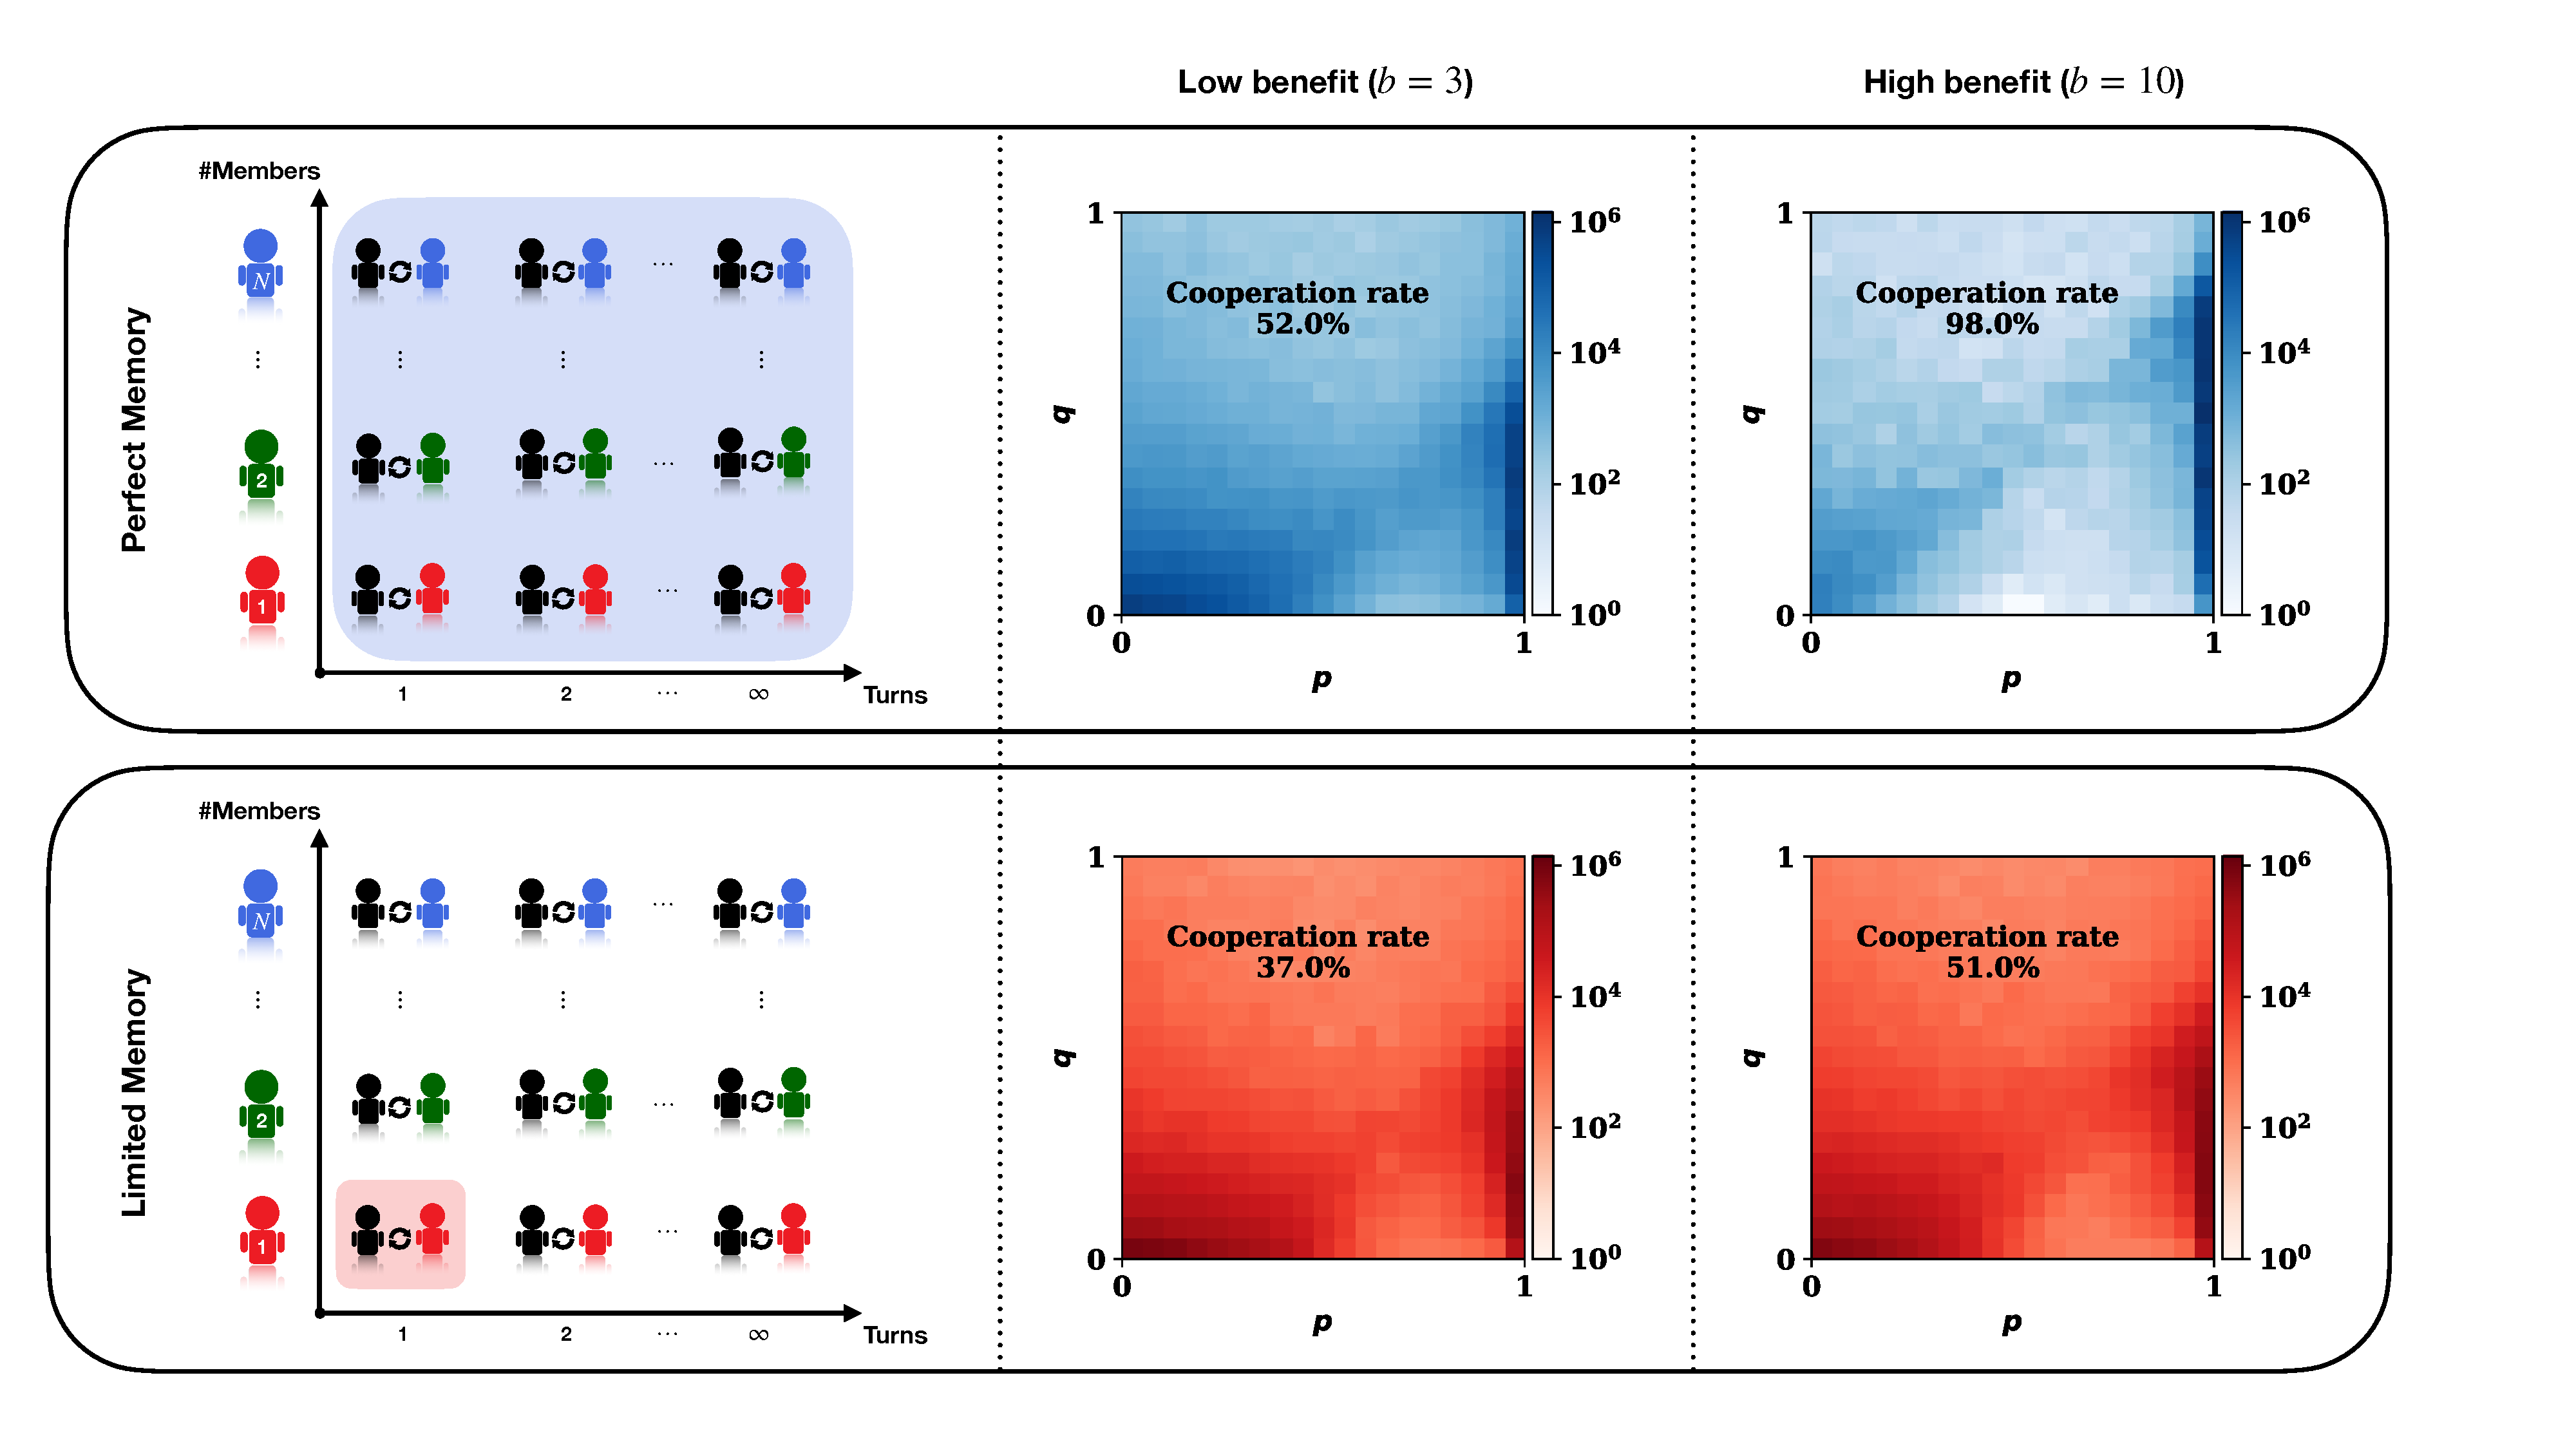
\includegraphics[width=\textwidth]{static/donation_expected_last_round_summary_results.pdf}
    \caption{{\bf Evolutionary dynamics under perfect and limited payoff memory.}
    ({\bf Schematic illustrations}) On the left panels we show schematic
    illustrations of the perfect memory and the limited memory cases. The shaded
    background denotes the game phase information that an individual considers
    when updating strategies. In the case of perfect payoff memory the entire region is
    shaded and in the case of limited payoff memory only one turn with a single member
    of the population. ({\bf Simulations}) We have run four simulations of the
    pairwise comparison process for $T\!=\!10^7$ time steps. For each time step
    of the process
    we record the current resident population ($y,p,q$). Since
    simulations are run for a relatively high continuation probability of
    $\delta\!=\!0.999$, we do not report the players' initial cooperation
    probability $y$. The plots show how often the resident population chooses
    each combination ($p,q$) of conditional cooperation probabilities in the
    subsequent rounds. We also report the evolved cooperation rate which is
    calculated as the average cooperation rate within the resident population.
    ({\bf Perfect Memory}) In the case of low benefit the resident population
    either consists of defectors (with $p\!\approx\!q\!\approx\!0$) or of
    conditional cooperators. Conditional cooperators, or otherwise known as
    generous tit for tat, are a set of strategies that always cooperate
    following a cooperation ($p\!\approx\!1\!$) and cooperate with a probability
    $q$ given that the co-player has defected. $q$ denotes the generosity of a
    player. The resident population applies a conditional cooperator strategy
    for which $q\!\le\!1\!-\!c/b\!=\!0.67$. 
    In the case of high benefit the population mainly consists of conditional
    cooperators of the form ($p\!\approx\!1\!, q\!\le\!1\!-\!1/10\!=\!0.9$). In
    the Supplementary Information Section 2 we show that a conditional
    cooperator needs to be of the form ($p\!\approx\!1\!, q\!\le\!1\!-\!c/b$) to
    not be invaded by defecting strategies. A higher generosity in the
    population results in a higher average cooperation rate. The average
    cooperation rate increases from 52\% for \(b=3\) to 98\% for \(b=10\). ({\bf
    Limited Memory}) When players update their strategies based on their
    realized payoffs in the last round, there are two different predominant
    behaviors regardless of the benefit value. The resident population either
    consists of defectors (with $p\!\approx\!q\!\approx\!0$) or of conditional
    cooperators. The maximum level of $q$, consistent with stable cooperation, is
    somewhat smaller compared to the perfect memory setting.
    Namely, in the Supplementary Information Section 3 we show that
    regardless of the value of benefit a conditional cooperator need to be of
    the form $q\!<\!\frac{1}{2}$ to not be invaded by defectors.
    The evolved cooperation
    rate only slightly increases from 37\% ($b=3$) to 51\% ($b=10$). Parameters: $N\!=\!100$,
    $c\!=\!1$, $\beta\!=\!1$, $\delta\!=\!0.999$.}
    \label{fig:expected_and_stochastic_for_donation}
\end{figure}

We further investigate the impact of benefit and selection strength on
generosity $q$ and the cooperation rate, as shown in Figure~\ref{fig:cooperation_rate_over_benefit_and_beta}.
According to Figure~\ref{fig:cooperation_rate_over_benefit_and_beta}\textbf{A},
perfect memory consistently results in a higher cooperation rate, which
increases with increasing benefit. On the other hand, the cooperation rate
remains approximately 50\% for limited payoff memory once \(b = 5\).
From Figure~\ref{fig:cooperation_rate_over_benefit_and_beta}\textbf{B}
we observe that for weak selection, \(\beta < 1\), the two methods yield similar
results, however, as \(\beta\) increases there is variation in the evolving
populations. In the case of expected payoffs the resident populations become
more cooperative, whereas in the case of limited payoff memory, the resident
populations become more defective.

\begin{figure}[!htbp]
    \centering
    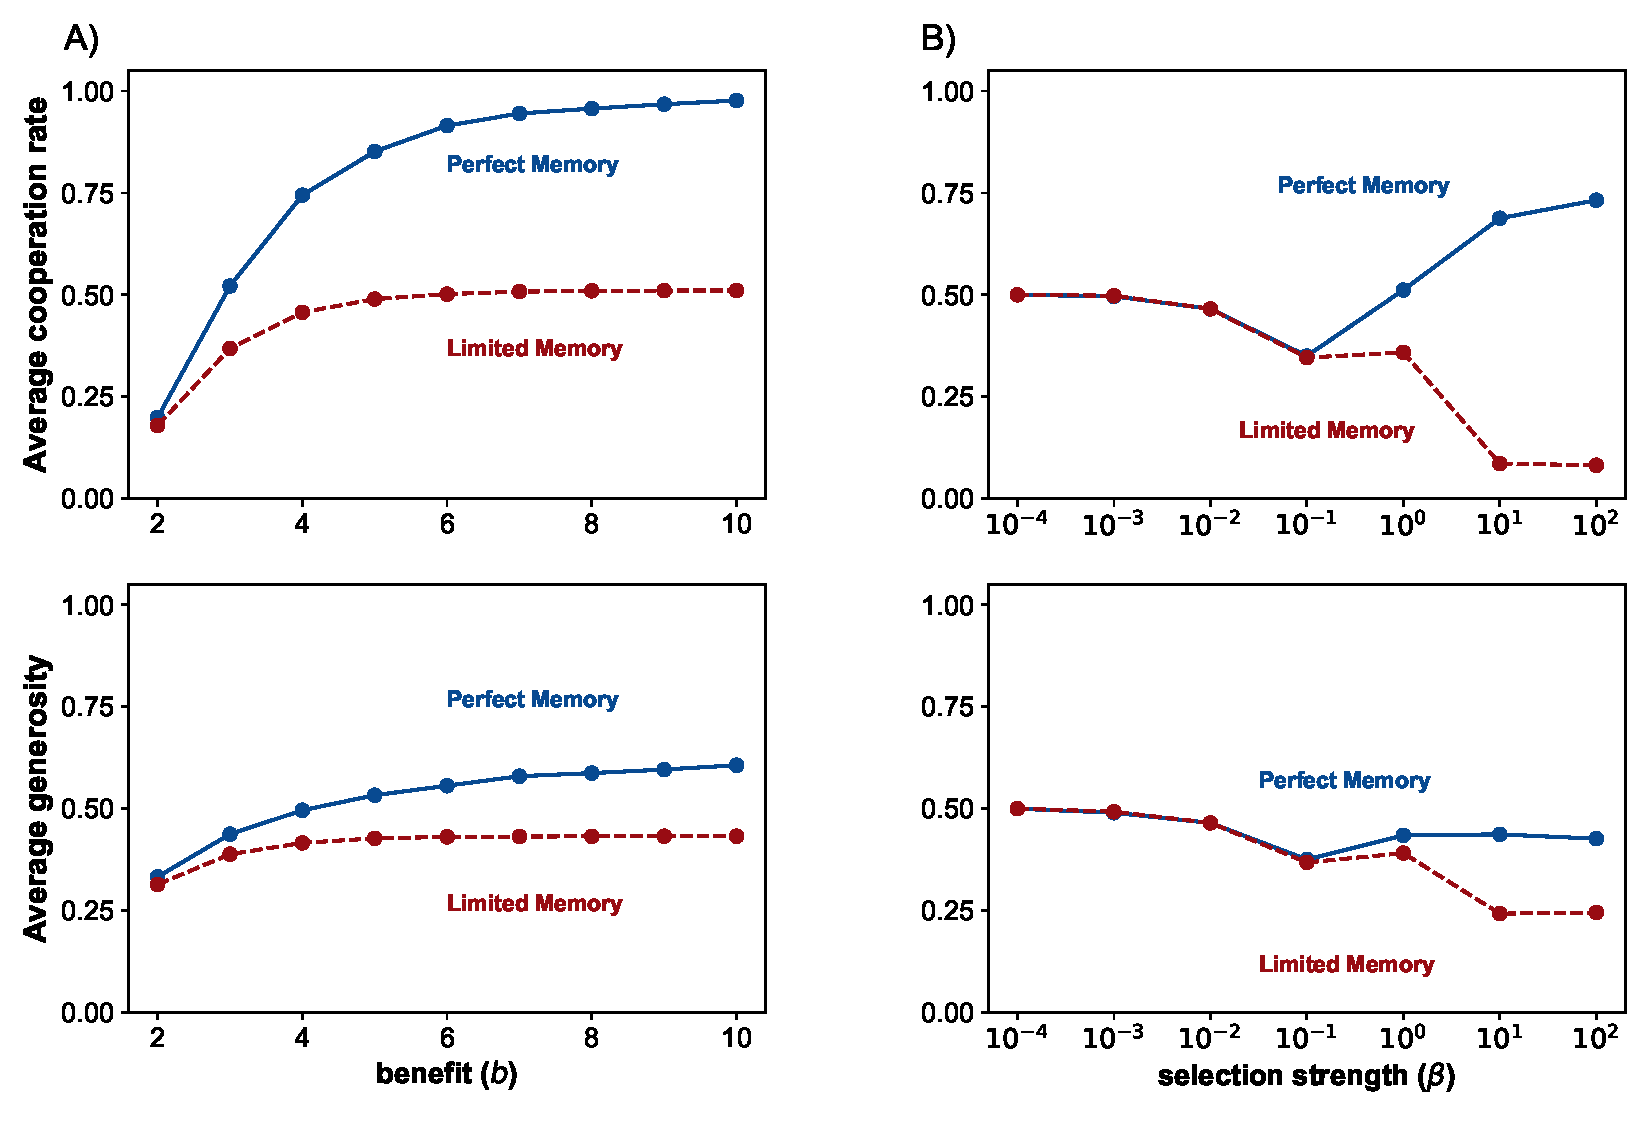
\includegraphics[width=.75\textwidth]{static/cooperation_rate_over_b_and_beta.pdf}
    \caption{{\bf The evolution of cooperation and generosity for different
    values of benefit (A) and strength of selection (B).} We report the average
    cooperation and the average reciprocity. The average cooperation rate is the
    average cooperation rate within the resident population. For the average
    reciprocity we select the residents that have a $p \approx 1$ and we take
    the average of their cooperation probability $q$. ({\bf A}) We vary the
    benefit of cooperation $b$. In all cases, perfect memory updating payoffs
    appear to overestimate the average cooperation rate the population achieves.
    As expected in the case of limited memory the average generosity over the
    different values of benefit remains the same ($q \approx 0.5$), and as a
    result so does the average cooperation. ({\bf B}) We vary the selection
    strength $\beta$. For weak selection, \(\beta < 1\), the two methods yield
    similar results. However, as \(\beta\) increases in the case of limited
    memory payoffs the resident populations become more defective. Note that
    in the case of perfect payoff memory we see an increase in the cooperation
    rate even though the generosity remains stable. That is because the
    generosity does remain the same, however, now cooperative strategies remain
    fixed as the resident strategy for longer.
    Unless
    explicitly varied, the parameters of the simulation are $N\!=\!100$,
    $b\!=\!3$, $c\!=\!1$, $\beta\!=\!1$, $\delta\!=\!0.99$. Simulations are run
    for $T\!=\!5\times 10^7$ time steps for each parameter
    combination.}\label{fig:cooperation_rate_over_benefit_and_beta}
\end{figure}

The limited payoff memory framework can be expanded by enabling individuals to
observe a greater number of rounds, interact with a larger number of members, or
both (refer to Supplementary Information Sections 4-6). To gain further insight
into the impact of limited payoff memory, we explore the scenarios of updating
based on the last round with two members of the population, the last two rounds
with another member of the population, and the last two rounds with two members
of the population. To analyze the effects of this framework, we conduct
numerical simulations using various fitness methods. The cooperation rates for
low and high benefits are presented in Figure~\ref{fig:cooperation_rate_all_updating_payoffs}.

We observe a significant rise in the cooperation rate with the introduction of
slightly more information. Specifically, in scenarios involving two rounds or
two interactions, the cooperation rates are almost identical. For a large
population and a high continuation probability ($\delta$), the conditional
cooperators that are adopted by the resident population in these scenarios take
on the same form \((1, q < \frac{\sqrt{2}}{2})\). When considering both sets
of information (i.e., two rounds and two interactions), cooperation rates
experience a greater increase, yet still remain lower compared to the classical
scenario.

\begin{figure}[!htbp]
  \centering
  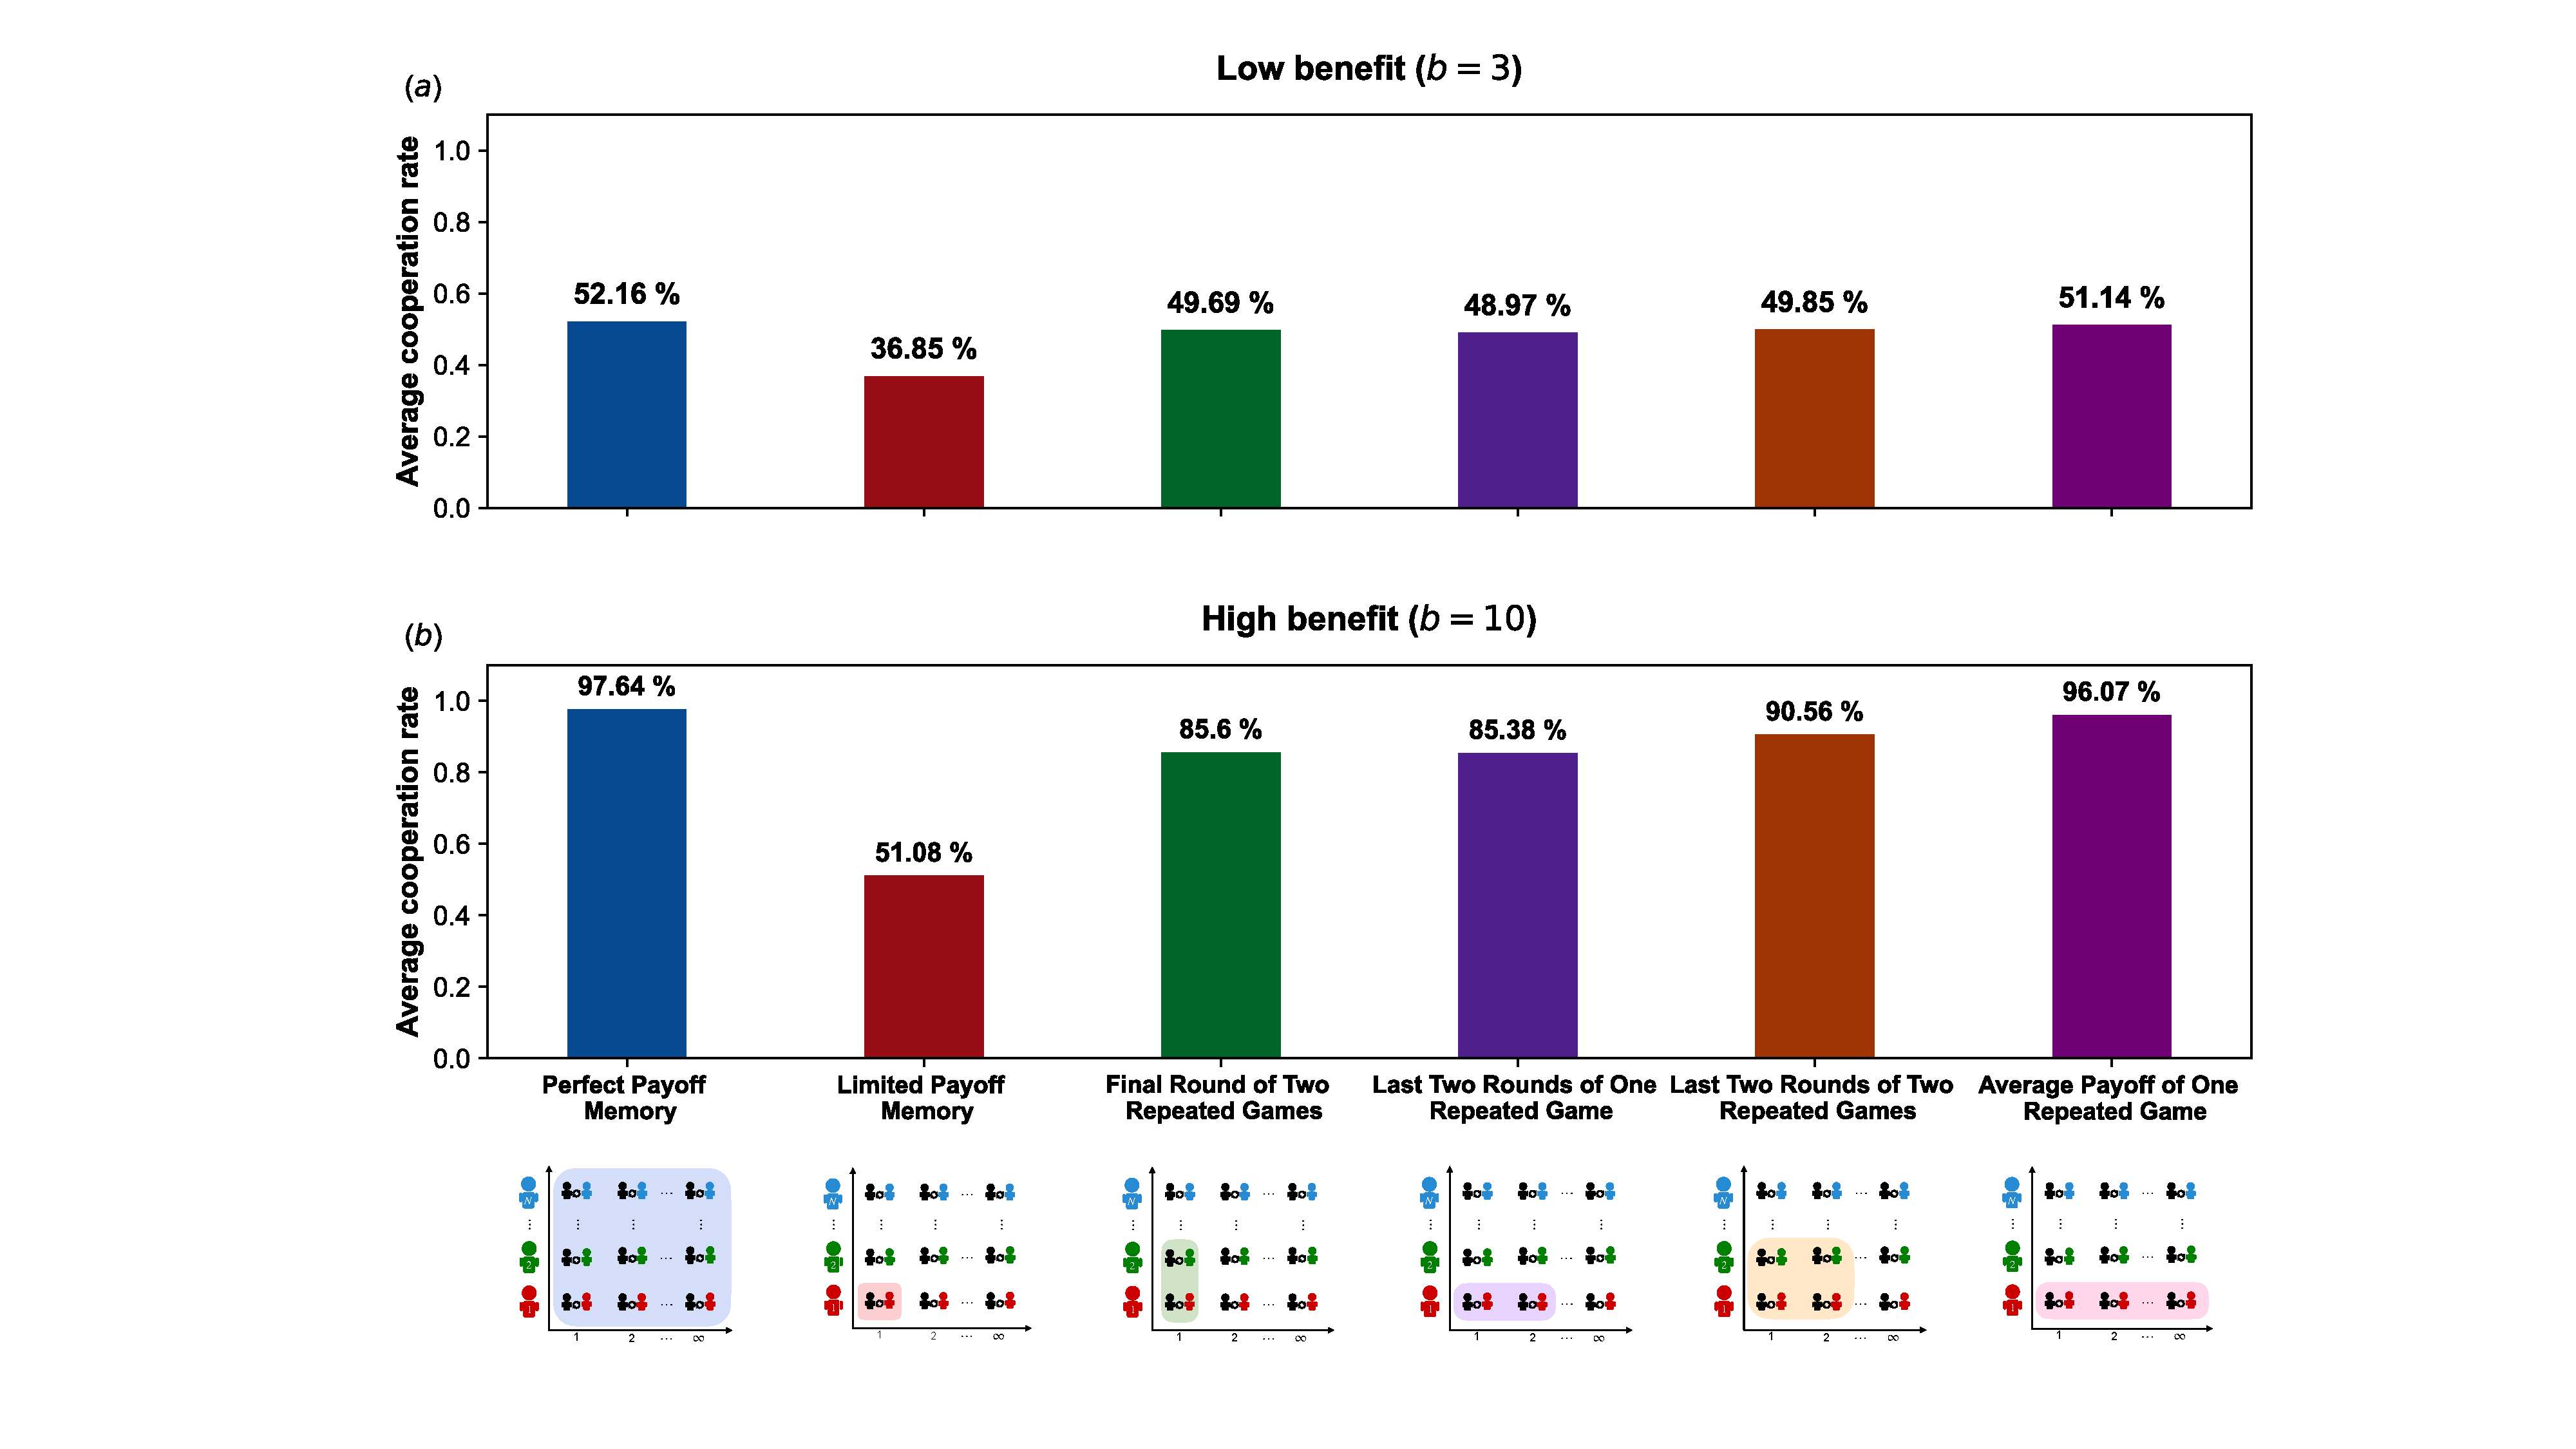
\includegraphics[width=\textwidth]{static/more_memory_summary_results.pdf}
  \caption{{\bf Average cooperation rates for different updating payoffs.}
  From left to right, we present result on the following updating payoffs cases;
  (a) the expected payoffs (perfect memory), (b) the last round payoff from one
  interaction (limited memory), (c) the last round payoff from two interactions,
  (d) the last two rounds payoffs from one interaction, (e) the last two rounds
  payoffs from two interactions. For the updating payoffs (c) and (d) we have
  carried out an analysis which has shown that conditional cooperators should
  adopt a \(q\) value smaller than $\frac{\delta - 1 +
  \frac{\sqrt{2}}{2}}{\delta}$ and $\frac{\delta + \sqrt{\delta^{2} + 1} - 1}{2 \delta}$
  respectively. Note that as \(\delta
  \rightarrow 1\) both right hand sides tend to \(\frac{\sqrt{2}}{2}\).
  Regardless the cooperation rate between for case (c) is slightly higher.
  In case (d) the cooperation rate is the second highest hinting that as we
  allow for more information the closer we move to the perfect payoff memory.
  We performed four pairwise non parametric tests (Mann-Whitney U) to compare
  the cooperation distributions of the residents in case (b) to
  cases (a), (c), (d), (e). In all four tests we reject the null hypothesis
  with \(\alpha=0.05\) and \(p \approx 0\). Thus, there is significant
  difference between the cooperation rates.
  Unless explicitly varied, the parameters of the simulation are
  $N\!=\!100$, $b\!=\!3$, $c\!=\!1$, $\beta\!=\!1$, $\delta\!=\!0.99$.
  Simulations are run for $T\!=\!5\times 10^7$ time steps for each parameter
  combination.}\label{fig:cooperation_rate_all_updating_payoffs}
\end{figure}

\section{Conclusions}\label{section:conclusions}

Cooperation can be seen as odd, why is it that we choose to help others at a
personal cost? In spite of all the selfish genes', animal and human communities
show signs of altruism and cooperation~\cite{milinski1987tit, kerr2002local,
carter2020development}. Evolutionary game theoretical models have helped us
shape our understanding of the evolution of cooperation. In fact, the evolution
of cooperation constitutes such a major focus of the field that evolutionary
game theory seems to be reduced to the evolution of
cooperation~\cite{Traulsen:PhilTrans:2022}. 

Evolutionary models in the past often feature a curious inconsistency. While
these models depict how individuals make decisions in each round by assuming
that they only retain memory of the previous round, they also assume that
individuals possess a perfect memory when it comes to updating their strategies
over time. To be precise, individuals are assumed to remember all of their past
interactions and each interaction's outcome when updating strategies.

Here, we investigate the robustness of cooperation as models deviate
from the assumption of perfect memory. While prior research has investigated the
impact of constraining individuals' interactions, we take into account the
limitation of not only interactions but also the information available for each
outcome. Additionally, prior studies have only allowed for the adoption of
simple strategies such as always cooperating or always defecting. In contrast,
we enable the use of more intricate strategies where players can utilize the
previous play of their co-player to make decisions.

In our framework, players update their strategies based on a combination of
interactions and outcomes. The initial scenario we examined involved using one
piece of information: the last round of one interaction. The outcomes suggest
that cooperation faces difficulties in developing when the updating stage
utilizes minimal social information. This effect is compounded as the benefit
and strength of selection are independently increased. The findings indicate
that cooperative players benefit from the ability to engage with all members of
the population.

Furthermore, we investigated scenarios where the final two rounds, or the last
two instances of interaction, were taken into account. We observed a
statistically significant rise in the frequency of cooperative behavior. For a
sizable population and a high likelihood of continued interactions, the two
cases yield the same result as the overall payoff is influenced by two possible
outcomes. Notably, the scenario involving two rounds and two interactions
yielded the highest cooperation rate among all the novel methodologies that we
tested.
% A nice sentence missing here.

\section{Acknowledgements}

This work was supported by the European Research Council Starting Grant 850529:
E-DIRECT.

\bibliographystyle{unsrt}
\bibliography{bibliography.bib}



\end{document}
